%! TeX program = xelatex
\documentclass[12pt, a4paper]{article}
\usepackage{geometry, tikz, float, pgfplots, xcolor, titlesec, amsmath, url, hanging, siunitx, graphicx, sectsty}
\usepackage[utf8]{inputenc}
\usepackage[skip=3pt]{parskip}
\usepackage[none]{hyphenat}
\usepackage[no-math]{fontspec}   % only changes normal font
% Tells LaTeX the images are kept in the "images" folder under the main directory
\graphicspath{ {./assets/} }
\pgfplotsset{compat=1.18, width=10cm}
% Spacing of sections: 0pt on the left, 18pt above, and 12pt below
\titlespacing\section{0pt}{18pt}{12pt}
% font size 12 for the sections
\sectionfont{\fontsize{12}{15}\selectfont}

% Setting font
\setromanfont{Arial}

% Setting strict margins
\sloppy

\begin{document}

\begin{center}

% Extra space at the top of the document
\noindent \\[10pt]
\color{black}

\thispagestyle{empty} % No page number for this page

\Large{\textbf{Properties of Gamma Radiation}} \\[30pt]
\normalsize \textit{Jack Greenberg, Jacob Fairham}\\[5pt]
\textit{11017146, 11074241}\\[20pt]
Department of Physics and Astronomy \\[5pt]
The University of Manchester \\[20pt]
First Year Laboratory Report 2 \\[20pt]
January 2023 \\[25pt]

\end{center}

\textbf{Abstract}\\[12pt]
This expirement aimed to analyze the spectra created using gamma ray spectroscopy using thallium-activated sodium iodide scintillation detectors with radioactive isotopes such as $^{22}$Na, $^{60}$Co, and $^{137}$Cs. The peaks of the $^{22}$Na spectrum were then used to calculate the strength of the sodium source and the relative efficiencies of the detector at the different photopeak energies, and then different materials were used between the isotopes and the detector to confirm the decay relation. We found our isotope of $^{22}$Na had a source strength of $11.77\pm1.81$kBq, as compared to its theoretical $15.09$kBq obtained using the initial source strength as well as the half life of the isotope and the amount of time that has passed from the initial source measurement.

\noindent 

\pagebreak

\section{Introduction}
		The boltzmann constant relates the average kinetic energy within a distribution of molecules to their temperature. Relating energy to temperature comes up in many contexts, from calculating how long to nuke or cook something to calculating how much thermal insulation a capsule returning to earth from the moon will need to survive reentry.

\section{Experimental Setup}
	\begin{figure}[H] \centering
		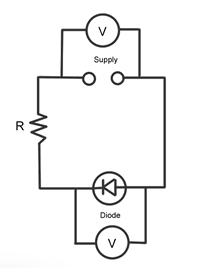
\includegraphics{assets/circdiag.png}
		\caption{Circut diagram}
	\end{figure}
	The power supply is hooked up on both ends to a voltmeter to ensure equipment quality. The negative end of the power supply is connected to both the diode voltmeter and the diode. The positive ends of both the diode and the voltmeter are connected to the input of the resistor. The output of the resistor is connected to both the power supply and the supply voltmeter.

\section{Theory}
	The current should be the same everywhere in the circuit assuming perfect voltmeters, and thus we can calculate the current over the semiconductor by calculating the current over the resistor by using equation 1.
	\begin{equation}
		I = \frac{V_s - V_d}{R}
		\label{eq. 1}
	\end{equation}
	where $V_s$ is the voltage being supplied to the circuit, $V_d$ is the voltage difference measured across the diode, $R$ is the resistance of our resistor in the circuit, and $I$ is the current in the circuit. The voltage drop across the resistor must be the difference in the supply voltage and the diode voltage by the loop rule. We can then compare this current to the theoretical current through a semiconductor$^{[1]}$
	\begin{equation}
		\ln [I] = \frac{e V_d}{kT} + \ln [I_0]
		\label{eq. 2}
	\end{equation}
	where $e$ is the absolute value of the charge of an electron, $k$ is the boltzmann constant, and $T$ is the temperature of the semiconductor. We can get the natural log of the voltage using equation 1, and we can take the derivative of equation 2 to obtain an equation for the Boltzmann Constant $k$
	\begin{equation}
		k = \frac{e}{T\frac{d[\ln [I]]}{dV_d}}
		\label{eq. 3}
	\end{equation}

\section{Procedure}
	We ultimately want to find the current as a function of the voltage in the circuit. We use the power supply to set the voltage and the variable resistor to set the restistance of the circut, and we can approximate the system as being ohmic. We use the setup shown in fig. 1 with the diode being a semiconductor, which, for our experiment, will be ice in a metal container. Our first measurements will be at 0 degrees celsius and at $10^3$ \si{\ohm}. We will collect data at all combinations of 0 and 100 degrees celsius and $10^3$, $10^4$, and $10^5$\si{\ohm}, varying the voltage on the integers from 1-30V inclusive. 

\section{Uncertainty Calculations}
	To calculate the uncertainty in the current, we use equation 2 as well as standard error propogation to get
	\begin{equation}
		\Delta [\ln [I]] = \sqrt{ \Big( \frac{\Delta V_s^2 - \Delta V_d^2}{V_s - V_d} \Big)^2 + \Big( \frac{\Delta R}{R} \Big)^2 }
		\label{eq. 4}
	\end{equation}
	\linebreak
	we know for our experiment that
	\begin{align*}
		\frac{\Delta R}{R} &= .01\\
		\frac{\Delta V_s}{V_s} &= .002\\
		\frac{\Delta V_d}{V_d} &= .002
	\end{align*}
	thus we can rewrite equation 4
	\begin{equation}
		\Delta [\ln [I]] = 10^{-2} \sqrt{ 4\times 10^{-2} \Big( \frac{V_s^2 + V_d^2}{V_s - V_d} \Big)^2 + 1 }
		\label{eq. 5}
	\end{equation}
	we can see that the factor of $4\times 10^{-2}$ will be a negligible contribution to the final uncertainty as long as $V_s - V_d$ is not too small or $V_s^2 + V_d^2$ is not too large, which turns out to be the case in practice based on our data. Thus we can approximate equation 5 as
	\begin{equation*}
		\Delta [\ln [I]] \approx .01
	\end{equation*}
	which we will then use to obtain an uncertainty for the derivative of the natural log of the current with respect to the diode voltage. Once that has been obtained through analysis of our data, we can calculate
	\begin{equation}
		\Delta k = k \sqrt{ \Big( \frac{\Delta [\frac{d[\ln[I]]}{dV_d}]}{\frac{d[\ln[I]]}{dV_d}} \Big)^2 + \Big( \frac{\Delta T}{T} \Big)^2 }
		\label{eq. 6}
	\end{equation}
	where we estimate the uncertainty in temperature to be
	\begin{equation*}
		\frac{\Delta T}{T} = .01
	\end{equation*}

\section{Data}
	Raw data is availible electronically$^{[2]}$. First, measurements were taken with the ice at $0^{\circ}$C, and we plotted the natural log of the current in the circuit as a function of the diode voltage, shown below. Error bars are small but plotted. Boltzmann constant calculated in SI units.
	\begin{figure}[H] \centering
		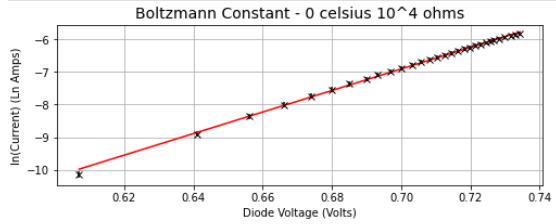
\includegraphics[scale=0.7]{assets/bcgraph_0c4o.png}
		\caption{Natural log of current by diode voltage, $0^{\circ}$C $10^4$\si{\ohm}}
	\end{figure}
	for this graph: $\frac{d[\ln [I]]}{dV_d} = 33.004 \pm 0.498$, and reduced $\chi^2 = 0.25$. Thus, $k = 1.7782 \times 10^{-23}$ and $\Delta k = 0.0322 \times 10^{-23}$.
	\begin{figure}[H] \centering
		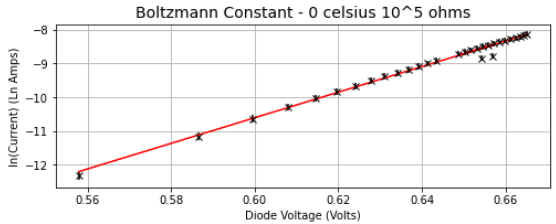
\includegraphics[scale=0.7]{assets/bcgraph_0c5o.png}
		\caption{Natural log of current by diode voltage, $0^{\circ}$C $10^5$\si{\ohm}}
	\end{figure}
	for this graph: $\frac{d[\ln [I]]}{dV_d} = 37.928 \pm 0.751$, and reduced $\chi^2 = 1.09$. Thus, $k = 1.5473 \times 10^{-23}$ and $\Delta k = 0.0343 \times 10^{-23}$.
	\begin{figure}[H] \centering
		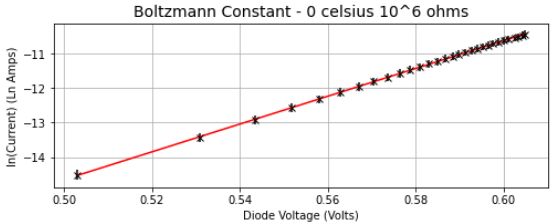
\includegraphics[scale=0.7]{assets/bcgraph_0c6o.png}
		\caption{Natural log of current by diode voltage, $0^{\circ}$C $10^6$\si{\ohm}}
	\end{figure}
	for this graph: $\frac{d[\ln [I]]}{dV_d} = 40.284 \pm 0.983$, and reduced $\chi^2 = 0.01$. Thus, $k = 1.4568 \times 10^{-23}$ and $\Delta k = 0.0384 \times 10^{-23}$.
	\linebreak
	Taking a weighted mean for the boltzmann constant for these graphs yields $k = 1.6120 \times 10^{-23}$ and $\Delta k = 0.0200 \times 10^{-23}$.
	\linebreak
	Next, the container was put on a hot plate and heated to $100^{\circ}$C, where the same measurements were taken, the graphs of which are shown below.
	\begin{figure}[H] \centering
		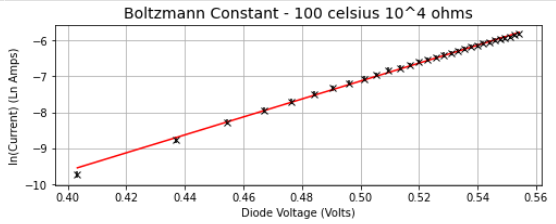
\includegraphics[scale=0.7]{assets/bcgraph_1c4o.png}
		\caption{Natural log of current by diode voltage, $100^{\circ}$C $10^4$\si{\ohm}}
	\end{figure}
	for this graph: $\frac{d[\ln [I]]}{dV_d} = 24.914 \pm 0.390$, and reduced $\chi^2 = 0.33$. Thus, $k = 1.7241 \times 10^{-23}$ and $\Delta k = 0.0320 \times 10^{-23}$.
	\begin{figure}[H] \centering
		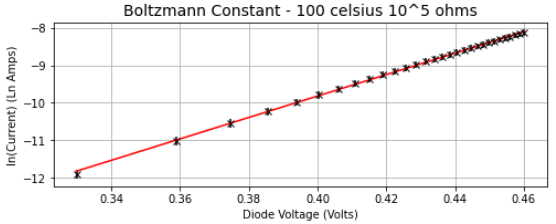
\includegraphics[scale=0.7]{assets/bcgraph_1c5o.png}
		\caption{Natural log of current by diode voltage, $100^{\circ}$C $10^5$\si{\ohm}}
	\end{figure}
	for this graph: $\frac{d[\ln [I]]}{dV_d} = 28.631 \pm 0.589$, and reduced $\chi^2 = 0.05$. Thus, $k = 1.5002 \times 10^{-23}$ and $\Delta k = 0.0343 \times 10^{-23}$.
	\begin{figure}[H] \centering
		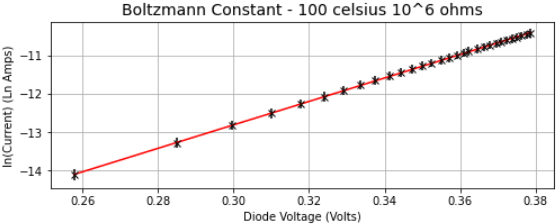
\includegraphics[scale=0.7]{assets/bcgraph_1c6o.png}
		\caption{Natural log of current by diode voltage, $100^{\circ}$C $10^6$\si{\ohm}}
	\end{figure}
	for this graph: $\frac{d[\ln [I]]}{dV_d} = 30.482 \pm 0.781$, and reduced $\chi^2 = 0.01$. Thus, $k = 1.4091 \times 10^{-23}$ and $\Delta k = 0.0388 \times 10^{-23}$.
	\linebreak
	\linebreak
	Taking a weighted mean for the boltzmann constant for these graphs yields $k = 1.5370 \times 10^{-23}$ and $\Delta k = 0.0200 \times 10^{-23}$. Taking a weighted mean for all the graphs at both temperatures yeilds $k = 1.5745 \times 10^{-23}$ and $\Delta k = 0.0141 \times 10^{-23}$.

\section{Analysis}
	As seen in the graphs, the diode voltage and current go down as the resistance increases. The slope of the graphs taken at $100^{\circ}C$ are significantly lower than those taken at $0^{\circ}$C, which makes sense given equation 3 - $k$ should remain constant, and thus if the temperature increases the slope should decrease. One thing we do see that is unexpected is that the slope increases quite significantly with the resistance. This is most likely due to us considering resistance from other areas in the circuit, like the wires, to be negligible. Thus, as the resistance from the resistor increases and becomes the dominant source of resistance in the circuit, we should get a value of the boltzmann constant closer to the value observed in other experiments, which we do find to be the case, as most other experiments put the value of the boltzmann constant around $1.38 \times 10^{-23}$ in SI units$^{[3]}$. 

\section{Conclusion}
	It is likely that we did not properly account for all sources of resistance in our calculations, such as resistance from the wires, because as the resistor becomes the dominant source of resistance making all other sources negligible our value for the boltzmann constant approaches the value measured in other experiments. Regardless, we were able to confirm the order of magnitude of the boltzmann constant, which allows us to describe, with moderate precision, the relationship between energy and temperature, which has uses that range from the kitchen to the architect's office. There are a couple of anomalous points but those are likely the result of a typo when taking the data as they only appear in figure 3. 

\section*{References}

	\begin{hangparas}{.25in}{1}
		[1] Ocaya, Richard. (2006). An experiment to profile the voltage, current and temperature behaviour of a P-N diode. European Journal of Physics. 27. 625. 10.1088/0143-0807/27/3/015.
		
		[2] Daussy, C. et al. "Direct Determination of the Boltzmann Constant by an Optical Method". Phys. Rev. Lett. 98. (2007): 250801.
	\end{hangparas}

\end{document}
